\documentclass{article}

% latex packages, feel free to add more here like 'tikz'
\usepackage{style/conference}
\usepackage{opensans}
\usepackage{graphicx}
\usepackage{biblatex}
\usepackage{fontawesome}
\usepackage[hidelinks]{hyperref}
\usepackage{subcaption}

% to reference, paste the BibTeX obtained from google scholar into references.bib
\addbibresource{references.bib}
%%%%% NEW MATH DEFINITIONS %%%%%

\usepackage{amsmath,amsfonts,bm}

% Mark sections of captions for referring to divisions of figures
\newcommand{\figleft}{{\em (Left)}}
\newcommand{\figcenter}{{\em (Center)}}
\newcommand{\figright}{{\em (Right)}}
\newcommand{\figtop}{{\em (Top)}}
\newcommand{\figbottom}{{\em (Bottom)}}
\newcommand{\captiona}{{\em (a)}}
\newcommand{\captionb}{{\em (b)}}
\newcommand{\captionc}{{\em (c)}}
\newcommand{\captiond}{{\em (d)}}

% Highlight a newly defined term
\newcommand{\newterm}[1]{{\bf #1}}


% Figure reference, lower-case.
\def\figref#1{figure~\ref{#1}}
% Figure reference, capital. For start of sentence
\def\Figref#1{Figure~\ref{#1}}
\def\twofigref#1#2{figures \ref{#1} and \ref{#2}}
\def\quadfigref#1#2#3#4{figures \ref{#1}, \ref{#2}, \ref{#3} and \ref{#4}}
% Section reference, lower-case.
\def\secref#1{section~\ref{#1}}
% Section reference, capital.
\def\Secref#1{Section~\ref{#1}}
% Reference to two sections.
\def\twosecrefs#1#2{sections \ref{#1} and \ref{#2}}
% Reference to three sections.
\def\secrefs#1#2#3{sections \ref{#1}, \ref{#2} and \ref{#3}}
% Reference to an equation, lower-case.
\def\eqref#1{equation~\ref{#1}}
% Reference to an equation, upper case
\def\Eqref#1{Equation~\ref{#1}}
% A raw reference to an equation---avoid using if possible
\def\plaineqref#1{\ref{#1}}
% Reference to a chapter, lower-case.
\def\chapref#1{chapter~\ref{#1}}
% Reference to an equation, upper case.
\def\Chapref#1{Chapter~\ref{#1}}
% Reference to a range of chapters
\def\rangechapref#1#2{chapters\ref{#1}--\ref{#2}}
% Reference to an algorithm, lower-case.
\def\algref#1{algorithm~\ref{#1}}
% Reference to an algorithm, upper case.
\def\Algref#1{Algorithm~\ref{#1}}
\def\twoalgref#1#2{algorithms \ref{#1} and \ref{#2}}
\def\Twoalgref#1#2{Algorithms \ref{#1} and \ref{#2}}
% Reference to a part, lower case
\def\partref#1{part~\ref{#1}}
% Reference to a part, upper case
\def\Partref#1{Part~\ref{#1}}
\def\twopartref#1#2{parts \ref{#1} and \ref{#2}}

\def\ceil#1{\lceil #1 \rceil}
\def\floor#1{\lfloor #1 \rfloor}
\def\1{\bm{1}}
\newcommand{\train}{\mathcal{D}}
\newcommand{\valid}{\mathcal{D_{\mathrm{valid}}}}
\newcommand{\test}{\mathcal{D_{\mathrm{test}}}}

\def\eps{{\epsilon}}


% Random variables
\def\reta{{\textnormal{$\eta$}}}
\def\ra{{\textnormal{a}}}
\def\rb{{\textnormal{b}}}
\def\rc{{\textnormal{c}}}
\def\rd{{\textnormal{d}}}
\def\re{{\textnormal{e}}}
\def\rf{{\textnormal{f}}}
\def\rg{{\textnormal{g}}}
\def\rh{{\textnormal{h}}}
\def\ri{{\textnormal{i}}}
\def\rj{{\textnormal{j}}}
\def\rk{{\textnormal{k}}}
\def\rl{{\textnormal{l}}}
% rm is already a command, just don't name any random variables m
\def\rn{{\textnormal{n}}}
\def\ro{{\textnormal{o}}}
\def\rp{{\textnormal{p}}}
\def\rq{{\textnormal{q}}}
\def\rr{{\textnormal{r}}}
\def\rs{{\textnormal{s}}}
\def\rt{{\textnormal{t}}}
\def\ru{{\textnormal{u}}}
\def\rv{{\textnormal{v}}}
\def\rw{{\textnormal{w}}}
\def\rx{{\textnormal{x}}}
\def\ry{{\textnormal{y}}}
\def\rz{{\textnormal{z}}}

% Random vectors
\def\rvepsilon{{\mathbf{\epsilon}}}
\def\rvtheta{{\mathbf{\theta}}}
\def\rva{{\mathbf{a}}}
\def\rvb{{\mathbf{b}}}
\def\rvc{{\mathbf{c}}}
\def\rvd{{\mathbf{d}}}
\def\rve{{\mathbf{e}}}
\def\rvf{{\mathbf{f}}}
\def\rvg{{\mathbf{g}}}
\def\rvh{{\mathbf{h}}}
\def\rvu{{\mathbf{i}}}
\def\rvj{{\mathbf{j}}}
\def\rvk{{\mathbf{k}}}
\def\rvl{{\mathbf{l}}}
\def\rvm{{\mathbf{m}}}
\def\rvn{{\mathbf{n}}}
\def\rvo{{\mathbf{o}}}
\def\rvp{{\mathbf{p}}}
\def\rvq{{\mathbf{q}}}
\def\rvr{{\mathbf{r}}}
\def\rvs{{\mathbf{s}}}
\def\rvt{{\mathbf{t}}}
\def\rvu{{\mathbf{u}}}
\def\rvv{{\mathbf{v}}}
\def\rvw{{\mathbf{w}}}
\def\rvx{{\mathbf{x}}}
\def\rvy{{\mathbf{y}}}
\def\rvz{{\mathbf{z}}}

% Elements of random vectors
\def\erva{{\textnormal{a}}}
\def\ervb{{\textnormal{b}}}
\def\ervc{{\textnormal{c}}}
\def\ervd{{\textnormal{d}}}
\def\erve{{\textnormal{e}}}
\def\ervf{{\textnormal{f}}}
\def\ervg{{\textnormal{g}}}
\def\ervh{{\textnormal{h}}}
\def\ervi{{\textnormal{i}}}
\def\ervj{{\textnormal{j}}}
\def\ervk{{\textnormal{k}}}
\def\ervl{{\textnormal{l}}}
\def\ervm{{\textnormal{m}}}
\def\ervn{{\textnormal{n}}}
\def\ervo{{\textnormal{o}}}
\def\ervp{{\textnormal{p}}}
\def\ervq{{\textnormal{q}}}
\def\ervr{{\textnormal{r}}}
\def\ervs{{\textnormal{s}}}
\def\ervt{{\textnormal{t}}}
\def\ervu{{\textnormal{u}}}
\def\ervv{{\textnormal{v}}}
\def\ervw{{\textnormal{w}}}
\def\ervx{{\textnormal{x}}}
\def\ervy{{\textnormal{y}}}
\def\ervz{{\textnormal{z}}}

% Random matrices
\def\rmA{{\mathbf{A}}}
\def\rmB{{\mathbf{B}}}
\def\rmC{{\mathbf{C}}}
\def\rmD{{\mathbf{D}}}
\def\rmE{{\mathbf{E}}}
\def\rmF{{\mathbf{F}}}
\def\rmG{{\mathbf{G}}}
\def\rmH{{\mathbf{H}}}
\def\rmI{{\mathbf{I}}}
\def\rmJ{{\mathbf{J}}}
\def\rmK{{\mathbf{K}}}
\def\rmL{{\mathbf{L}}}
\def\rmM{{\mathbf{M}}}
\def\rmN{{\mathbf{N}}}
\def\rmO{{\mathbf{O}}}
\def\rmP{{\mathbf{P}}}
\def\rmQ{{\mathbf{Q}}}
\def\rmR{{\mathbf{R}}}
\def\rmS{{\mathbf{S}}}
\def\rmT{{\mathbf{T}}}
\def\rmU{{\mathbf{U}}}
\def\rmV{{\mathbf{V}}}
\def\rmW{{\mathbf{W}}}
\def\rmX{{\mathbf{X}}}
\def\rmY{{\mathbf{Y}}}
\def\rmZ{{\mathbf{Z}}}

% Elements of random matrices
\def\ermA{{\textnormal{A}}}
\def\ermB{{\textnormal{B}}}
\def\ermC{{\textnormal{C}}}
\def\ermD{{\textnormal{D}}}
\def\ermE{{\textnormal{E}}}
\def\ermF{{\textnormal{F}}}
\def\ermG{{\textnormal{G}}}
\def\ermH{{\textnormal{H}}}
\def\ermI{{\textnormal{I}}}
\def\ermJ{{\textnormal{J}}}
\def\ermK{{\textnormal{K}}}
\def\ermL{{\textnormal{L}}}
\def\ermM{{\textnormal{M}}}
\def\ermN{{\textnormal{N}}}
\def\ermO{{\textnormal{O}}}
\def\ermP{{\textnormal{P}}}
\def\ermQ{{\textnormal{Q}}}
\def\ermR{{\textnormal{R}}}
\def\ermS{{\textnormal{S}}}
\def\ermT{{\textnormal{T}}}
\def\ermU{{\textnormal{U}}}
\def\ermV{{\textnormal{V}}}
\def\ermW{{\textnormal{W}}}
\def\ermX{{\textnormal{X}}}
\def\ermY{{\textnormal{Y}}}
\def\ermZ{{\textnormal{Z}}}

% Vectors
\def\vzero{{\bm{0}}}
\def\vone{{\bm{1}}}
\def\vmu{{\bm{\mu}}}
\def\vtheta{{\bm{\theta}}}
\def\va{{\bm{a}}}
\def\vb{{\bm{b}}}
\def\vc{{\bm{c}}}
\def\vd{{\bm{d}}}
\def\ve{{\bm{e}}}
\def\vf{{\bm{f}}}
\def\vg{{\bm{g}}}
\def\vh{{\bm{h}}}
\def\vi{{\bm{i}}}
\def\vj{{\bm{j}}}
\def\vk{{\bm{k}}}
\def\vl{{\bm{l}}}
\def\vm{{\bm{m}}}
\def\vn{{\bm{n}}}
\def\vo{{\bm{o}}}
\def\vp{{\bm{p}}}
\def\vq{{\bm{q}}}
\def\vr{{\bm{r}}}
\def\vs{{\bm{s}}}
\def\vt{{\bm{t}}}
\def\vu{{\bm{u}}}
\def\vv{{\bm{v}}}
\def\vw{{\bm{w}}}
\def\vx{{\bm{x}}}
\def\vy{{\bm{y}}}
\def\vz{{\bm{z}}}

% Elements of vectors
\def\evalpha{{\alpha}}
\def\evbeta{{\beta}}
\def\evepsilon{{\epsilon}}
\def\evlambda{{\lambda}}
\def\evomega{{\omega}}
\def\evmu{{\mu}}
\def\evpsi{{\psi}}
\def\evsigma{{\sigma}}
\def\evtheta{{\theta}}
\def\eva{{a}}
\def\evb{{b}}
\def\evc{{c}}
\def\evd{{d}}
\def\eve{{e}}
\def\evf{{f}}
\def\evg{{g}}
\def\evh{{h}}
\def\evi{{i}}
\def\evj{{j}}
\def\evk{{k}}
\def\evl{{l}}
\def\evm{{m}}
\def\evn{{n}}
\def\evo{{o}}
\def\evp{{p}}
\def\evq{{q}}
\def\evr{{r}}
\def\evs{{s}}
\def\evt{{t}}
\def\evu{{u}}
\def\evv{{v}}
\def\evw{{w}}
\def\evx{{x}}
\def\evy{{y}}
\def\evz{{z}}

% Matrix
\def\mA{{\bm{A}}}
\def\mB{{\bm{B}}}
\def\mC{{\bm{C}}}
\def\mD{{\bm{D}}}
\def\mE{{\bm{E}}}
\def\mF{{\bm{F}}}
\def\mG{{\bm{G}}}
\def\mH{{\bm{H}}}
\def\mI{{\bm{I}}}
\def\mJ{{\bm{J}}}
\def\mK{{\bm{K}}}
\def\mL{{\bm{L}}}
\def\mM{{\bm{M}}}
\def\mN{{\bm{N}}}
\def\mO{{\bm{O}}}
\def\mP{{\bm{P}}}
\def\mQ{{\bm{Q}}}
\def\mR{{\bm{R}}}
\def\mS{{\bm{S}}}
\def\mT{{\bm{T}}}
\def\mU{{\bm{U}}}
\def\mV{{\bm{V}}}
\def\mW{{\bm{W}}}
\def\mX{{\bm{X}}}
\def\mY{{\bm{Y}}}
\def\mZ{{\bm{Z}}}
\def\mBeta{{\bm{\beta}}}
\def\mPhi{{\bm{\Phi}}}
\def\mLambda{{\bm{\Lambda}}}
\def\mSigma{{\bm{\Sigma}}}

% Tensor
\DeclareMathAlphabet{\mathsfit}{\encodingdefault}{\sfdefault}{m}{sl}
\SetMathAlphabet{\mathsfit}{bold}{\encodingdefault}{\sfdefault}{bx}{n}
\newcommand{\tens}[1]{\bm{\mathsfit{#1}}}
\def\tA{{\tens{A}}}
\def\tB{{\tens{B}}}
\def\tC{{\tens{C}}}
\def\tD{{\tens{D}}}
\def\tE{{\tens{E}}}
\def\tF{{\tens{F}}}
\def\tG{{\tens{G}}}
\def\tH{{\tens{H}}}
\def\tI{{\tens{I}}}
\def\tJ{{\tens{J}}}
\def\tK{{\tens{K}}}
\def\tL{{\tens{L}}}
\def\tM{{\tens{M}}}
\def\tN{{\tens{N}}}
\def\tO{{\tens{O}}}
\def\tP{{\tens{P}}}
\def\tQ{{\tens{Q}}}
\def\tR{{\tens{R}}}
\def\tS{{\tens{S}}}
\def\tT{{\tens{T}}}
\def\tU{{\tens{U}}}
\def\tV{{\tens{V}}}
\def\tW{{\tens{W}}}
\def\tX{{\tens{X}}}
\def\tY{{\tens{Y}}}
\def\tZ{{\tens{Z}}}


% Graph
\def\gA{{\mathcal{A}}}
\def\gB{{\mathcal{B}}}
\def\gC{{\mathcal{C}}}
\def\gD{{\mathcal{D}}}
\def\gE{{\mathcal{E}}}
\def\gF{{\mathcal{F}}}
\def\gG{{\mathcal{G}}}
\def\gH{{\mathcal{H}}}
\def\gI{{\mathcal{I}}}
\def\gJ{{\mathcal{J}}}
\def\gK{{\mathcal{K}}}
\def\gL{{\mathcal{L}}}
\def\gM{{\mathcal{M}}}
\def\gN{{\mathcal{N}}}
\def\gO{{\mathcal{O}}}
\def\gP{{\mathcal{P}}}
\def\gQ{{\mathcal{Q}}}
\def\gR{{\mathcal{R}}}
\def\gS{{\mathcal{S}}}
\def\gT{{\mathcal{T}}}
\def\gU{{\mathcal{U}}}
\def\gV{{\mathcal{V}}}
\def\gW{{\mathcal{W}}}
\def\gX{{\mathcal{X}}}
\def\gY{{\mathcal{Y}}}
\def\gZ{{\mathcal{Z}}}

% Sets
\def\sA{{\mathbb{A}}}
\def\sB{{\mathbb{B}}}
\def\sC{{\mathbb{C}}}
\def\sD{{\mathbb{D}}}
% Don't use a set called E, because this would be the same as our symbol
% for expectation.
\def\sF{{\mathbb{F}}}
\def\sG{{\mathbb{G}}}
\def\sH{{\mathbb{H}}}
\def\sI{{\mathbb{I}}}
\def\sJ{{\mathbb{J}}}
\def\sK{{\mathbb{K}}}
\def\sL{{\mathbb{L}}}
\def\sM{{\mathbb{M}}}
\def\sN{{\mathbb{N}}}
\def\sO{{\mathbb{O}}}
\def\sP{{\mathbb{P}}}
\def\sQ{{\mathbb{Q}}}
\def\sR{{\mathbb{R}}}
\def\sS{{\mathbb{S}}}
\def\sT{{\mathbb{T}}}
\def\sU{{\mathbb{U}}}
\def\sV{{\mathbb{V}}}
\def\sW{{\mathbb{W}}}
\def\sX{{\mathbb{X}}}
\def\sY{{\mathbb{Y}}}
\def\sZ{{\mathbb{Z}}}

% Entries of a matrix
\def\emLambda{{\Lambda}}
\def\emA{{A}}
\def\emB{{B}}
\def\emC{{C}}
\def\emD{{D}}
\def\emE{{E}}
\def\emF{{F}}
\def\emG{{G}}
\def\emH{{H}}
\def\emI{{I}}
\def\emJ{{J}}
\def\emK{{K}}
\def\emL{{L}}
\def\emM{{M}}
\def\emN{{N}}
\def\emO{{O}}
\def\emP{{P}}
\def\emQ{{Q}}
\def\emR{{R}}
\def\emS{{S}}
\def\emT{{T}}
\def\emU{{U}}
\def\emV{{V}}
\def\emW{{W}}
\def\emX{{X}}
\def\emY{{Y}}
\def\emZ{{Z}}
\def\emSigma{{\Sigma}}

% entries of a tensor
% Same font as tensor, without \bm wrapper
\newcommand{\etens}[1]{\mathsfit{#1}}
\def\etLambda{{\etens{\Lambda}}}
\def\etA{{\etens{A}}}
\def\etB{{\etens{B}}}
\def\etC{{\etens{C}}}
\def\etD{{\etens{D}}}
\def\etE{{\etens{E}}}
\def\etF{{\etens{F}}}
\def\etG{{\etens{G}}}
\def\etH{{\etens{H}}}
\def\etI{{\etens{I}}}
\def\etJ{{\etens{J}}}
\def\etK{{\etens{K}}}
\def\etL{{\etens{L}}}
\def\etM{{\etens{M}}}
\def\etN{{\etens{N}}}
\def\etO{{\etens{O}}}
\def\etP{{\etens{P}}}
\def\etQ{{\etens{Q}}}
\def\etR{{\etens{R}}}
\def\etS{{\etens{S}}}
\def\etT{{\etens{T}}}
\def\etU{{\etens{U}}}
\def\etV{{\etens{V}}}
\def\etW{{\etens{W}}}
\def\etX{{\etens{X}}}
\def\etY{{\etens{Y}}}
\def\etZ{{\etens{Z}}}

% The true underlying data generating distribution
\newcommand{\pdata}{p_{\rm{data}}}
% The empirical distribution defined by the training set
\newcommand{\ptrain}{\hat{p}_{\rm{data}}}
\newcommand{\Ptrain}{\hat{P}_{\rm{data}}}
% The model distribution
\newcommand{\pmodel}{p_{\rm{model}}}
\newcommand{\Pmodel}{P_{\rm{model}}}
\newcommand{\ptildemodel}{\tilde{p}_{\rm{model}}}
% Stochastic autoencoder distributions
\newcommand{\pencode}{p_{\rm{encoder}}}
\newcommand{\pdecode}{p_{\rm{decoder}}}
\newcommand{\precons}{p_{\rm{reconstruct}}}

\newcommand{\laplace}{\mathrm{Laplace}} % Laplace distribution

\newcommand{\E}{\mathbb{E}}
\newcommand{\Ls}{\mathcal{L}}
\newcommand{\R}{\mathbb{R}}
\newcommand{\emp}{\tilde{p}}
\newcommand{\lr}{\alpha}
\newcommand{\reg}{\lambda}
\newcommand{\rect}{\mathrm{rectifier}}
\newcommand{\softmax}{\mathrm{softmax}}
\newcommand{\sigmoid}{\sigma}
\newcommand{\softplus}{\zeta}
\newcommand{\KL}{D_{\mathrm{KL}}}
\newcommand{\Var}{\mathrm{Var}}
\newcommand{\standarderror}{\mathrm{SE}}
\newcommand{\Cov}{\mathrm{Cov}}
% Wolfram Mathworld says $L^2$ is for function spaces and $\ell^2$ is for vectors
% But then they seem to use $L^2$ for vectors throughout the site, and so does
% wikipedia.
\newcommand{\normlzero}{L^0}
\newcommand{\normlone}{L^1}
\newcommand{\normltwo}{L^2}
\newcommand{\normlp}{L^p}
\newcommand{\normmax}{L^\infty}

\newcommand{\parents}{Pa} % See usage in notation.tex. Chosen to match Daphne's book.

\DeclareMathOperator*{\argmax}{arg\,max}
\DeclareMathOperator*{\argmin}{arg\,min}

\DeclareMathOperator{\sign}{sign}
\DeclareMathOperator{\Tr}{Tr}
\let\ab\allowbreak


% replace this title with your own
\title{Generating Pegasus with a MMD-VAE and semi-supervised learning}

\begin{document}
\maketitle
\begin{abstract}
    This paper proposes using a MMD-VAE, semi-supervised learning and latent space interpolation to generate images that look like a Pegasus. MMD Variation Auto Encoders are similar to conventional VAE but replace KL-loss for MMD-loss, helping to combat several issues faced by VAEs. The MMD-VAE is used in an unsupervised learning process to create a latent space encoder and decoder for the CIFAR-10 dataset. Linear interpolation between labeled horse and bird images is then employed to create a pegasus image. This method is enhanced using a semi-supervised \footnote{Although technically this isn't semi-supervised learning as it requires a fully labeled dataset like CIFAR-10. Given such a dataset the author uses a problem specific semi-supervised technique within the labeled dataset.} learning technique where the author selects "ideal" horse and bird images. These ideal images are then used to create subclasses within the horse and bird classes. These subclasses are used to enhance the interpolation process.

\end{abstract}

% this is where the sections begin
\section{Architecture}
\begin{center}
    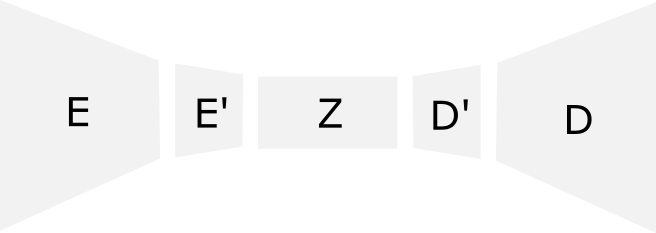
\includegraphics[width=0.5\textwidth]{figures/Encoder.png}
\end{center}
The encoder decoder has the conventional shape of an Auto Encoder.
The encoder is comprised of E and E' where E follows a ResNet \cite{ResNet} architecture with 18 convolution layers as decribeed by He. et al. E' is 3 fully connected layers linearly reducing in size in logspace from the output size of the ResNet to latent space size inspired by Barua et al's work on fully connected convolutional GANs \cite{fccGAN}. A MMD-VAE, unlike a VAE, samples directly from the encoder rather than from an encoder's mean and std output fields. Hence, you do not see an intermediate layer of means and stds. The latent space Z is 256 dimensions. 

The decoder is a mirror image of the encoder. It is comprised of 3 fully connected layers D', upscaling to D. D is also based of the ResNet-18 architecture however where a conventional ResNet would scale down at the end of a convolutional layer D scales up.



\begin{center}
    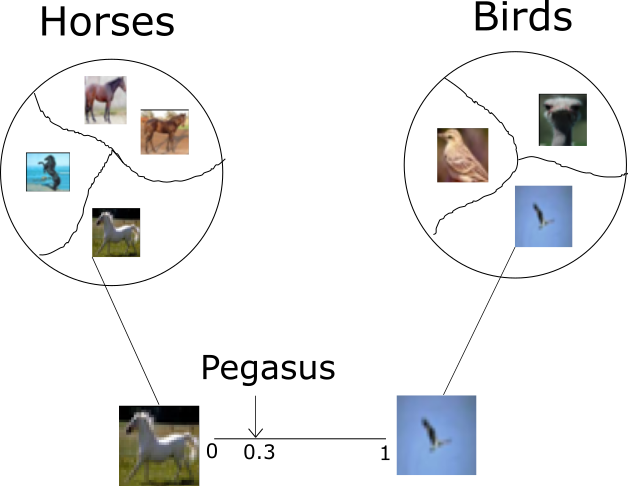
\includegraphics[width=0.45\textwidth]{figures/clustering.png}
\end{center}

Once the MMD-VAE is trained the horse and bird classes are subclassified and a pegasus generated through linear interpolation.

\section{Methodology}
The network reduces the MMD-VAE loss function \cite{infovae}. 
There are 2 terms in the MMD-VAE loss function. Firstly, the reconstruction loss:
\begin{equation}
    \mathcal{L}_{\textrm{recon}} = \mathbb{E}_{p_{\textrm{data}}(x)} \mathbb{E}_{q_\phi (z|x)} [\log p_\theta(x|z)]
\end{equation}

Where $\mathbb{E}[p_\theta(x|z)]$ is approximated by networks D' and D, parameterized by $\theta$ and likewise $\mathbb{E}[q_\phi(z|x)]$ is approximated by networks E and E', parameterized by $\phi$.


Secondly the Maximum Mean Discrepancy \cite{mmd}. Which is used to fit latent codes $z$ to prior $p(z)$.
\begin{equation}
    \textrm{MMD}(p(z) \lVert q(z)) = \mathbb{E}_{p(z), p_(z')}[k(z, z')] + \mathbb{E}_{q(z), q_(z')}[k(z, z')] - 2 \mathbb{E}_{p(z), q_(z')}[k(z, z')]
\end{equation}
where $k(z, z')$ is the gaussian kernel: $k(z, z')={\rm e}^{-\frac{\lVert z-z' \rVert^2}{2\sigma^2}}$

The full loss function is:
\begin{equation}
    \mathcal{L}_\textrm{MMD-VAE} = \lambda \cdot \textrm{MMD}(q_\phi (z) \lVert p(z)) + \mathcal{L}_{\textrm{recon}}
\end{equation}

where $q_\phi(z) =  \mathbb{E}[q_\phi(z|x)]$ and $\lambda$ is a scaling constant.

Batches of horse and bird images are then subclassified to create an improved dataset of horse and bird images. Random images from these dataset are then lineally interpolated between in latent space and the result decoded to create a pegasus image. 

\section{Class subclassification}
There is a huge variety of horse and bird images in CIFAR-10. Some images contain useful features such as white horses or bird wings. Others images predominantly contain unhelpful features such as beaks. Linear interpolation is very sensitive to input images so selecting better horse and bird images will help produce better pegasus. To do this I use semi-supervised learning. Firstly, I clustered a sample of horse or bird pictures in latent space using k-means. Then, using a handful of ideal horse/bird images (\ref{fig:good_horses}), I selected the "ideal" clusters which should contain many similar features to the example images. If the ideal images fall in different cluster I take the union of these cluster.

I also experimented with clustering over the union of 2 classes and creating subclasses from the intersection/difference of these classes. The idea being different classes may share features. For example, the intersection of birds and planes could be wings. The difference between cats and birds could be the set of birds excluding bird faces. Although an interesting idea, clusters were mainly formed around global features such as background colour. With this in mind, I found I got better subclassification using the semi-supervised learning approach.


\begin{figure}
    \begin{center}
    \begin{subfigure}{.2\textwidth}
    \begin{center}
        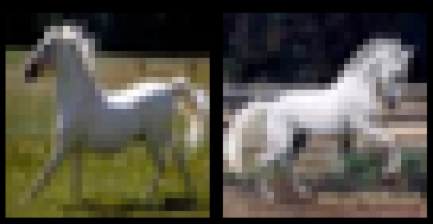
\includegraphics[width=.95\textwidth]{figures/good_horses_cropped.png}
    \end{center}
    \caption{"Ideal" white horses}
\end{subfigure}
\begin{subfigure}{.7\textwidth}
    \begin{center}
        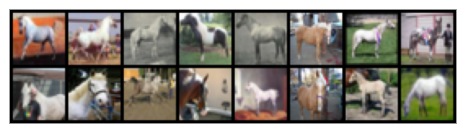
\includegraphics[width=.95\textwidth]{figures/white_horse_class.png}
    \end{center}
    \caption{Corresponding cluster}
\end{subfigure}
\caption{Using selected images to create subclasses}
    \label{fig:good_horses}
\end{center}
\end{figure}

\section{Results}
The best batch of pegasus images looks like this:
\begin{center}
    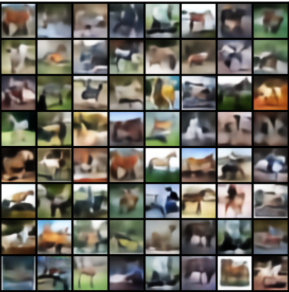
\includegraphics[width=0.5\textwidth]{figures/64_cropped.png}
\end{center}
From this batch, the most Pegasus-like image is:
\begin{center}
    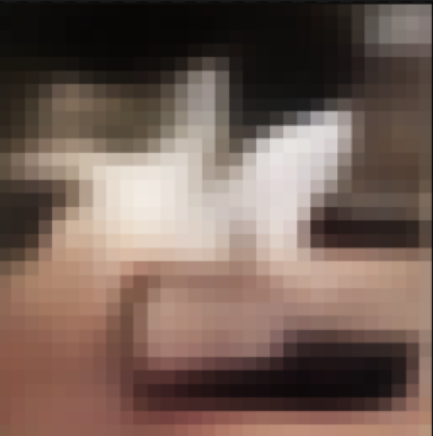
\includegraphics[width=0.1\textwidth]{figures/1_cropped.png}
\end{center}

As you can see there is a wide range of pegasuses. Some look rather good like and others are complete non-sense. Using linear interpolation made the output pegasus very sensitive to its' 2 input images. Although, subclassification improved this it certainly didn't solve the issue.

There are many brown pegasus in the batch because one of the ideal horses match to a very large, predominantly brown, horse cluster.

\section{Limitations}
The encoder failed to recreate fine details and textures. I suspect this is a confounding error accumulating through: the overkill ResNet architecture; basic data preparation; basic training strategy; and insufficient training time for the size of the network.

The subclassification of images was noisy, so although it reduced the domain of horse and bird images it didn't entirely remove unwanted images like ostriches (of which CIFAR-10 contains many).

Finally, the method of linear interpolation between a horse and a bird to create a pegasus is fundamental flawed. A pegasus is a horse with wings, not a bird-horse amalgam. This is talked about more in the improvements section.  



\section{Possible Improvements}
There may be some scope for improvement by \textbf{tweaking the ResNet} construction. In the interest of time I used the exact construction as described by He et al \cite{ResNet}. However, making the ResNet shallower would have helped to speed up training hence more training could have been done in a limited time frame. Also, given that the described architecture was developed for the 112x112 ImageNet images it's likely not as well suited for 32x32 CIFAR-10 images. In particular the initial 7x7 convolution is likely too large given I only had the opportunity to train on CIFAR-10.

\textbf{Cylindrical anealing} of MMD loss. The model uses the constant $\lambda=1$ for the MMD loss. This leads to vanishing MMD loss, much like VAEs suffer vanishing KL-loss. Fu et al \cite{cylindricalAnnealing} proposed a simple technique of cylindrically annealing $\lambda$. They showed this could substantially improve reconstruction error. I suspect that cylindrical annealing would have similar benefits for MMD-VAEs.

\textbf{Data preparation} could have been improved. I used random horizontal flips of the data but didn't have time to explore any other data preparation techniques. For example introducing color jitter may have helped the VAE to learn more color specific latent features which may have helped improve subclasses. Also random crops and scales may have helped the VAE better learn features such as wings. Also random crops and scales would help the model learn a degree of scale invariance which would open the door to doing transfer learning on STL-10.  

The use of \textbf{subclasses} definitely enhanced the final pegasus. However, there is still a lot of room for improvement. Firstly, sampling could be improved. Taking the union of ideal sets results in larger sets, like brown horses, dominating the final pegasus. A probabilistic sampling approach would solve this issue. Secondly, subclasses often shared global features such as background. Creating subclasses using randomly permuted (cropped, scaled, e.t.c.) data may lead to many more feature specific subclasses.

\textbf{Replacing interpolation} would help a lot with creating better pegasuses. If you extracted the latent representation of a wing and then applied this to the latent representation of a horse you would likely generate better pegasuses. You could extract the latent representation of a wing using class/subclass similarities. Then there are many methods you could use to apply this wing to a horse, from simple addition, to interpolation, to sampling based methods.


\section*{Bonuses}
This submission has a total bonus of -2 marks as it is only trained on CIFAR-10.

% you can have an unlimited number of references (they can go on the 5th page and span many additional pages without any penalty)
\printbibliography
\end{document}